\section{Планувальники у розподілених обчисленнях}

Планувальники в загальному поділяются на два типи: статичні та динамічні. Статичні мають певне правило розподілу задач на обчислювальні вузли та правило не зміюється під час роботи планувальника. Динамічні планувальники в свою чергу можуть адаптуватися під час роботи та змінювати стратегії планування. Хоч динамічні планувальники і здаються більш універсальними, проте вони дуже складні для аналізу та часто розробляються з метою оптимізації певного параметра.

Основною метою планування є розподіл виконання задач, які надсилають користувачі, між обчислювальними вузлами. Планувальник формує чергу виконання задач, та визначає яку задачу на якому вузлі стартувати. Частіше за все користувачів хвилює лише мінімізація часу завершення деякої відправленої множини задач у хмару.

Структура хмари у загальному випадку описується за допомоги таких сутностей як:
\begin{itemize}
	\item брокер
	\item планувальник
	\item дата центр
	\item хост
	\item віртуальна машина
\end{itemize}

Брокер являєься посередником між користувачем та хмарою і саме він формує запити до хмари на виконання задач та отримує результати їх виконання. Планувальник отримує задачі від брокерів різних користувачів та має свою певну стратегію розподілу черги задач, саме він керує дата центрами. Дата центри це несамостійні сутності і повністю керовані планувальниками. Їх основна мета - надавати обчислювальні вузли, запускати задачі по команді від планувальника та віддавати результати. Також у випадку динамічної хмари по певним запитам вони можуть збільшувати чи зменшувати кількість обчислювальних вузлів у мережі.
Віртуальна машина - це окремий обчислювальний вузол, який вміє лише отримувати вхідні дані, виконувати задачу та відправляти результат у дата центр.

\begin{figure}[H]
	\centering
	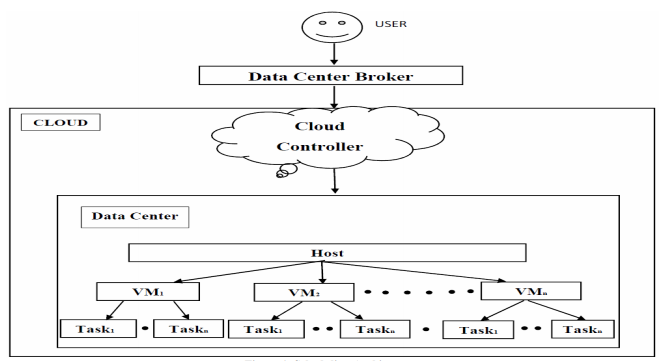
\includegraphics[width=\textwidth]{task_analysis/img/cloud_representation}
	\caption{Ілюстрація структури хмарної обчислювальної мережі}
	\label{fig:cloud_representation}
\end{figure}

Існує дві політики планування: space shared та time shared. У політиці space shared задачі у черзі розділяють між собою логічні ядра процесора обчислювального вулза і у випадку якщо усі ядра зайняті, то задач чекає звільнення ядра. Саме ця політика і вікористовується для тестування алгоритмів планування оскільки у випадку коли обчислювальні вузли мають лише одне ядро процесора, задачі виконуються послідовно від початку до кінця. Найпростіший алгоритм, який можна зустріти разом з політикою space shared - first come first served (FCFS).

Етапи роботи space shared політики:
\begin{itemize}
	\item[Крок 1] Формується черга задач
	\item[Крок 2] Запланувати виконання наступної задачі із черги
	\item[Крок 3] При завершенні задачі відправити результат
	\item[Крок 4] Якщо черга непорожня, то повернутися на крок 2
	\item[Крок 5] Кінець
	\item[***] Нові отримані задачі просто додаються у чергу і вони чекають свого виконання
\end{itemize}

Time shared політика в свою чергу означає що задачі у чергі розділяють між собою процесорний час. Тобто не обчислювальні ресурси, а проміжки часу які будуть витрачені на виконання кожної із задач. Усі задачі в черзі стартують в один і той самий час. Задача планувальника в цьому випадку - вирішувати коли потрібно призупинити виконання одної задачі та стартувати чи продовжити виконання іншої задачі. На перший погляд ця політика значно краща оскільки дозволяє виконувати набір задач поступово, проте час переключення від одної задачі до другої також потрібно враховувати. А також щоб стартувати усі задачі потрібно мати вхідні дані для усіх задач, що також не завжди зручно. Разом з цією політикою часто можна зустріти посилання на алгоритм планування Round Robin.

Етапи роботи tune shared політики:
\begin{itemize}
	\item[Крок 1] Формується черга задач.
	\item[Крок 2] Усі задачі запускаються одночасно у режимі переключення між задачами за правилом, яке визначає планувальник
	\item[Крок 3] Кінець
	\item[***] Нові отримані задачі просто додаються у чергу і зразу запускаються та працюють у режимі спільного використання процесорного часу
\end{itemize}

\begin{figure}[H]
	\centering
	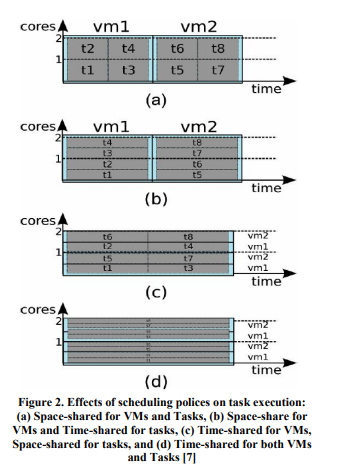
\includegraphics[width=\textwidth]{task_analysis/img/time_space_shared}
	\caption{Ілюстрація планування задач для time та space shared }
	\label{fig:time_space_shared}
\end{figure}

